\documentclass[tikz]{standalone}
\usetikzlibrary{positioning, arrows.meta}

\begin{document}
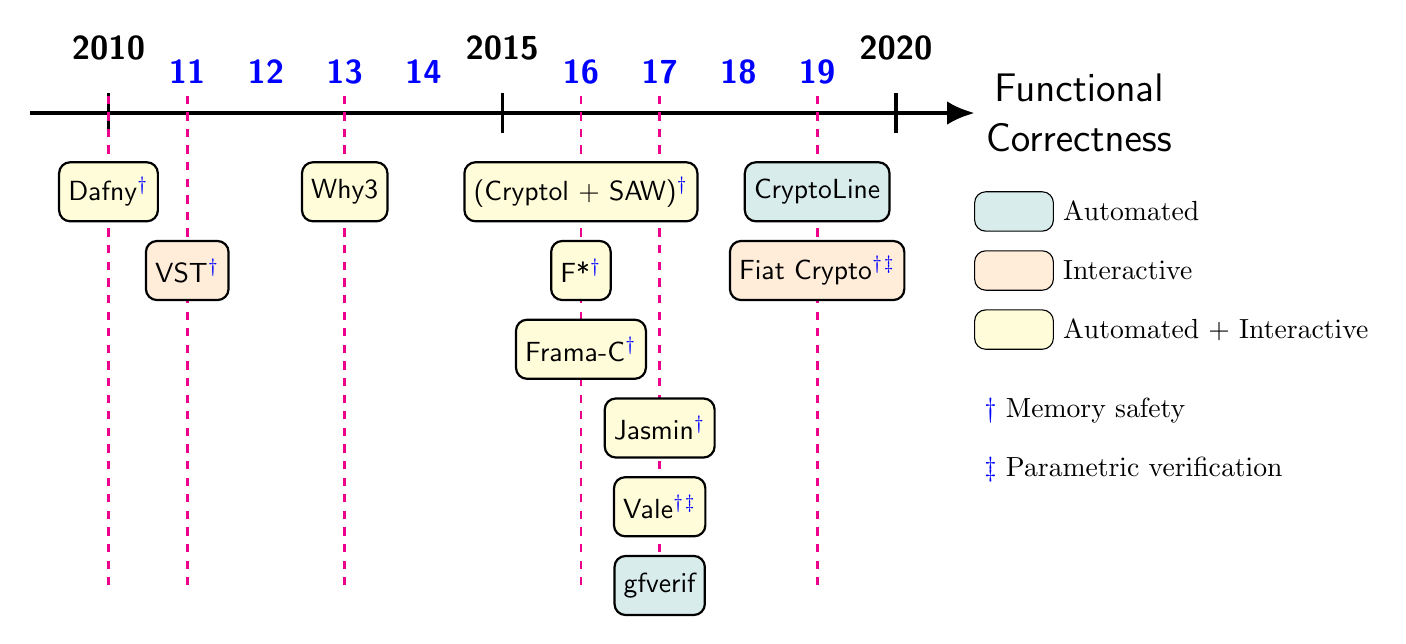
\begin{tikzpicture}[
	% Define a node distance for consistent spacing
	node distance=1cm and 2cm,
	% Style for the event description boxes
	event/.style={
		rectangle,
		rounded corners=4pt,
		draw=black,
		thick,
		fill=blue!20,
		text width=6cm,
		align=center,
		font=\sffamily,
		minimum height=1cm
	},
	event2/.style={
		rectangle,
		rounded corners=4pt,
		draw=black,
		thick,
		fill=orange!20,
		text width=8cm,
		align=center,
		font=\sffamily,
		minimum height=1cm
	},
	event3/.style={
		rectangle,
		rounded corners=4pt,
		draw=black,
		thick,
		fill=teal!20,
		text width=8cm,
		align=center,
		font=\sffamily,
		minimum height=1cm
	},
	% Style for the year markers on the axis
	year/.style={
		font=\sffamily\bfseries\large,
		anchor=south
	},
	node/.style={
		rectangle,
		rounded corners=4pt,
		draw=black,
		thick,
		fill=white,
%		text width=8cm,
		align=center,
		font=\sffamily,
		minimum height=.75cm
	},
	unbounded/.style={
		rectangle,
		rounded corners=4pt,
		draw=black,
		thick,
		fill=teal!15,
		align=center,
		font=\sffamily,
		minimum height=.75cm
	},
	bounded/.style={
		rectangle,
		rounded corners=4pt,
		draw=black,
		thick,
		fill=orange!15,
		align=center,
		font=\sffamily,
		minimum height=.75cm
	},
	equiv/.style={
		rectangle,
		rounded corners=4pt,
		draw=black,
		thick,
		fill=yellow!15,
		align=center,
		font=\sffamily,
		minimum height=.75cm
	}
	]
	% Draw the main horizontal timeline axis with a nice arrow tip
	\draw[line width=1.5pt, -{Latex[length=3.5mm, width=3mm]}] (4,0) -- (16,0) node[right, font=\Large\sffamily, align=center] {Functional\\ Correctness};
	
	\draw[fill=teal!15, rounded corners=4pt] (16,-1.5) rectangle (17,-1) node[below right] {Automated};
	\draw[fill=orange!15, rounded corners=4pt] (16,-2.25) rectangle (17,-1.75) node[below right] {Interactive};
	\draw[fill=yellow!15, rounded corners=4pt] (16,-3) rectangle (17,-2.5) node[below right] {Automated + Interactive};
	\draw[draw=white, rounded corners=4pt] (15,-4) rectangle (16,-3.5) node[below right] {$\color{blue}{\dagger}$ Memory safety};
	\draw[draw=white, rounded corners=4pt] (15,-4.75) rectangle (16,-4.25) node[below right] {$\color{blue}{\ddagger}$ Parametric verification};
	
	% Use a loop to place the years and tick marks on the axis
	\foreach \x/\yeartext in {5/2010, 10/2015, 15/2020}{
		\draw[line width=1.2pt] (\x, -0.25) -- (\x, 0.25);
		\node[year, above=0.3cm of {\x,0.25}] {\yeartext};
	}
	
	% Position the event nodes relative to coordinates on the timeline
%	\draw[red, fill=red] (8,0) circle (2.5pt) node[below=.25cm] {NOW};
	\node[year, above=0cm of {6,0.25}, blue] {11};
	\node[year, above=0cm of {7,0.25}, blue] {12};
	\node[year, above=0cm of {8,0.25}, blue] {13};
	\node[year, above=0cm of {9,0.25}, blue] {14};
	\node[year, above=0cm of {11,0.25}, blue] {16};
	\node[year, above=0cm of {12,0.25}, blue] {17};
	\node[year, above=0cm of {13,0.25}, blue] {18};
	\node[year, above=0cm of {14,0.25}, blue] {19};
	
	\foreach \x in {5,6,8,11,12,14}{
		\draw[line width=1pt, dashed, magenta] (\x, -6) -- (\x, 0.25);
	}
%	\draw[line width=1.5pt, dashed, blue] (-1, -6) -- (-1, 0.25);
%	\draw[line width=1.5pt, dashed, blue] (0, -6) -- (0, 0.25);
	
	\node[equiv] (CS)at (11,-1) {(Cryptol + SAW)$\color{blue}^{\dagger}$}; % 16
	\node[unbounded] (CL) at (14,-1) {CryptoLine}; % 19
	\node[equiv] (Da) at (5,-1) {Dafny$\color{blue}^{\dagger}$}; % 10
	\node[equiv] (F)at (11,-2) {F*$\color{blue}^{\dagger}$}; % 16
	\node[bounded] (FC) at (14,-2) {Fiat Crypto$\color{blue}^{\dagger}$$\color{blue}^{\ddagger}$}; % 19
	\node[equiv] (Fm) at (11,-3) {Frama-C$\color{blue}^{\dagger}$}; % 16
	\node[unbounded] (gf) at (12,-6) {gfverif}; % 17
	\node[equiv] (Ja) at (12,-4) {Jasmin$\color{blue}^{\dagger}$}; % 17
	\node[equiv] (Va1) at (12,-5) {Vale$\color{blue}^{\dagger}$$\color{blue}^{\ddagger}$}; % 17
%	\node[unbounded] (Va2) at (14,-3) {Vale}; % 19
	\node[bounded] (VS) at (6,-2) {VST$\color{blue}^{\dagger}$}; % 11
	\node[equiv] (Wh) at (8,-1) {Why3}; % 13
	
%	\draw[line width=1.5pt] (F7.east) to (F5.west);
%	\draw[line width=1.5pt] (Tamarin.east) -| (SAPIC.north);
%	\draw[line width=1.5pt] (fs2pv.east) -| (StatVerif.west);
%	\draw[line width=1.5pt] (StatVerif.east) -| (ProVerif.west);
%	\draw[line width=1.5pt] (ProVerif.east) -| (GSVerif.west);
%	\draw[line width=1.5pt] (GSVerif.east) -| (ProVerif-ATP.north);
	
\end{tikzpicture}
\end{document}